\section{Hauptteil}
\subsection{Projektmeilensteine}
Zu Projektbeginn wurden eine Reihe von Meilensteinen definiert, welche zeitgebundene Ziele repräsentieren, die zu spezifizierten Zeitpunkten erreicht werden sollten. Die Natur dieser Ziele reicht von eher grundlegenden Aufgaben, etwa der Evaluierung von Frameworks für Linux, Windows und Android, bis hin zu anspruchsvolleren und diversifizierten Zielen, wie etwa der Implementierung von Nachrichtenversand und Anruf-Funktionalitäten. Die vollständige Auflistung der definierten Meilensteine ist im ersten Anhang einsehbar.\\
Gemäss der Meilensteinplanung galt die initiale Aufgabe der Erlangung von Kompetenzen in Go bezüglich der GUI-Entwicklung. Für das Windows-Framework fiel die Wahl auf Wails \cite{wails}, während für Linux GTK als geeignet erachtet wurde. Ursprünglich war die Verwendung von QT \cite{qt} für Linux vorgesehen, jedoch stellten Kompilationsprobleme aufgrund von Inkompatibilitäten mit dem angestrebten, jedoch veralteten Framework ein Hindernis dar. Folglich wurde Gogtk3 \cite{gogtk3} als Ersatz ausgewählt.
\subsection{Funktionen, Datentypen und Variablen in Go}
\subsubsection{Eine Einführung in die diversen Variablentypen in Go}
Go bietet eine Vielzahl an Variablentypen, einschliesslich Zeichenketten (Strings), Ganzzahlen (Integers) und vorzeichenlosen Ganzzahlen (Unsigned Integers). Im Folgenden erfolgt ein Versuch, diese in einer möglichst zugänglichen und prägnanten Form zu erklären.

Zeichenketten (Strings)\\
In Go kann ein String jeden beliebigen Wert repräsentieren, nicht notwendigerweise UTF-8 kodiert, sondern jeglichen vorstellbaren Wert.

Ganzzahl (Integer)\\
Ein Integer hingegen ist auf Zahlenwerte innerhalb eines definierten Bereichs begrenzt. Hierbei ist zu berücksichtigen, ob ein int8 (Byte), int16, int32 oder int64 definiert wird, da jeder dieser Typen einen spezifischen Wertebereich umfasst. Ein int8 erstreckt sich von -128 bis 127, ein int16 von -32'768 bis 32'767, ein int32 von -2'147'483'648 bis 2'147'483'647 und ein int64 von -9'223'372'036'854'775'808 bis 9'223'372'036'854'775'807.

Vorzeichenlose Ganzzahlen (Unsigned Integers)\\
Darüber hinaus existieren vorzeichenlose Ganzzahlen, die lediglich Werte grösser oder gleich Null speichern können und deren Wertebereich jeweils von 0 bis zur Summe aus der negativen und der positiven Zahl der entsprechenden Integer-Typen reicht.\\
Es existieren darüber hinaus auch Gleitkommazahlen, Slices und zahlreiche weitere Typen. Für detailliertere Informationen wird auf die Golang-Spezifikationen\footnote{Golang-Spezifikationen: https://go.dev/ref/spec} verwiesen.
\subsubsection{Deklaration und Verwendung von Variablen in Go}
Die Methodik zur Deklaration von Variablen in Go offeriert eine Vielzahl an Möglichkeiten. Eine Deklaration der Variable könnte beispielsweise auf folgende Art und Weise erfolgen:
\begin{lstlisting}
var name string
\end{lstlisting}
Obiges Codefragment demonstriert die Deklaration einer String-Variable mit dem Namen "name". Um sie innerhalb eines Programms einzusetzen, könnte folgende Implementierung herangezogen werden:
\begin{lstlisting}
name = fmt.Sprintf("Cedric")
\end{lstlisting}
Trotzdem war dieser Ansatz eher sporadisch in Gebrauch, da es notwendig war, im Voraus den Typ der Variable festzulegen. In den meisten Fällen wurde daher die dynamische Variablendeklaration verwendet, welche eine Variable des Typs "string" unter dem Namen "name" wie nachstehend definiert:
\begin{lstlisting}
name := fmt.Sprintf("Cedric")
\end{lstlisting}
\subsubsection{Deklaration und Verwendung von Funktionen in Go}
Die Deklaration einer Funktion in Go erfordert die Verwendung des Schlüsselworts "func", gefolgt vom Namen der Funktion. Für eine Funktion namens "helloWorld" könnte die Formulierung beispielsweise so aussehen:
\begin{lstlisting}
func helloWorld() {}
\end{lstlisting}
Die runden Klammern repräsentieren die Parameterliste, die geschweiften Klammern den Funktionskörper. Zur Hinzufügung eines Parameters vom Typ String mit dem Namen "name", welcher mit "Hallo" kombiniert und zurückgegeben wird, sähe der zugehörige Code folgendermassen aus:
\begin{lstlisting}
func helloWorld(name string) {
    fmt.Printf("Hallo, %s", name)
}
\end{lstlisting}
Dies ist eine Funktion, die lediglich den Namen auf der Standardausgabe ausgibt. Es besteht jedoch auch die Möglichkeit, dass Funktionen Werte zurückgeben. In diesem Fall muss der Rückgabewert in der Funktionsdeklaration angegeben und vorab mit dem Schlüsselwort "return" notiert werden, was etwa so aussehen könnte:
\begin{lstlisting}
func helloWorld(name string) string {
    return fmt.Sprintf("Hallo, %s", name)
}
\end{lstlisting}
\subsection{Erste Schritte}
Die anfängliche Aufgabe war geprägt von der Recherche zu GUI-Frameworks. Die darauf folgende Aufgabe bestand in der Erstellung einer rudimentären Anwendung mit einem Texteingabefeld.
\begin{figure}[!ht]
\centering
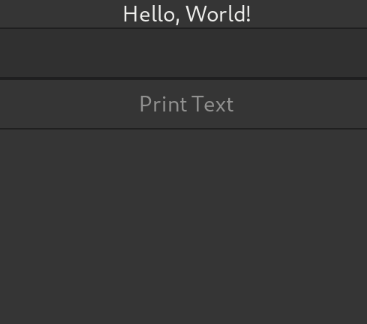
\includegraphics[width=0.5\textwidth]{txt/pictures/simple_window.png}
\caption{Ein GTK-Fenster, das ein Textfeld beinhaltet.}
\label{fig:example}
\end{figure}
Die Einfachheit stand im Fokus des ersten Programms, welches den Text aus dem Eingabefeld auf stdout ausgibt.
\subsection{Entscheidung bezüglich der GUI}
\subsubsection{Wails als GUI Framework}
Für eine gewisse Zeitperiode wurde das GUI-Entwicklungswerkzeug Wails favorisiert, jedoch erfolgte keine abschliessende Entscheidung zu dessen Gunsten. Nichtsdestotrotz konnte die existierende Gtk-Anwendung innerhalb von lediglich zwei Stunden komplett umgestaltet werden - ein Prozess, der mit Gtk insgesamt drei Tage in Anspruch genommen hat. Ein weiterer Vorteil von Wails ist die Möglichkeit, JavaScript und HTML zur Gestaltung des Fensters zu verwenden. Zusätzlich bietet Wails eine geschätzte Funktion namens 'Automatische Neukompilierungen' \cite{wailsAutoRebuild}, welche Änderungen am Code vornimmt und das Programm automatisch aktualisiert. Von Linux aus ist es zudem einfacher, für Windows und MacOSX zu kompilieren. In einem späteren Abschnitt werde ich detaillierter auf die Gründe eingehen, warum ich von Wails zu Fyne gewechselt bin.
\subsubsection{Fyne als GUI-Framework}
Die finale Entscheidung fiel zugunsten von Fyne \cite{fyne-web}, welches nun auch finanziell unterstützt wird (siehe Anhang 2 für den Beleg), da es durch herausragende Eigenschaften überzeugen konnte. Die Verwendung eines Frameworks, das meinen Code nicht in eine andere Sprache kompiliert, ermöglicht die Nutzung aller Go-Funktionen und -Bibliotheken. Dies ebnet den Weg für die Erstellung komplexerer Anwendungen. Darüber hinaus erlaubt Fyne nicht nur die Kompilierung für Windows/Linux, wie bei Wails, sondern auch für Android. Dies hat den Vorteil, dass lediglich eine Codebasis gepflegt werden muss, anstatt zwei separate zu unterhalten.
\subsection{Erstes Projekt}
Das erste Projekt unter Verwendung des Wails-Frameworks war eine einfache plattformübergreifende Wetter-App, die die OpenWeatherAPI verwendet. Die App ist ausschliesslich für die Stadt Winterthur verfügbar, da es schwierig ist, den GPS-Standort in Go zu ermitteln, und dies auch nicht in dem Projekt benötigt wird, da dies die Privatsphäre einschränkt.
\subsection{Verschlüsselungs-Stack}
Der geplante Verschlüsselungs-Stack soll die folgenden Algorithmen verwenden: \hyperref[glo:blake]{\(blake2b\_512^{[d]}\)}, \hyperref[glo:ecc]{\(ECC^{[e]}\)}, \hyperref[glo:aes]{\(AES^{[f]}\)} und \hyperref[glo:crystal-dilithium]{\(CRYSTAL-Dilithium^{[g]}\)}.
\\
Die Entscheidung für einen derart komplexen Verschlüsselungs-Stack fiel aufgrund des hohen Stellenwerts von Sicherheit und Privatsphäre innerhalb meines Messengers. Dementsprechend wurde ein Algorithmus integriert, der auch gegenüber Angriffen durch Quantencomputer zuverlässig ist. Es ist sehr wichtig, gegen zukünftige Angriffsmethoden so gut wie möglich geschützt zu sein.
\\
Die Wahl fiel auf den CRYSTAL-Dilithium-Algorithmus, da dieser vom NIST empfohlen wird. \cite{nist-recomedation}
\subsubsection{Erstellung des Entschlüsselungsmoduls}
Das Ziel bestand darin, ein möglichst modulares Entschlüsselungsmodul zu erstellen. Daher war geplant, das Modul mit zahlreichen Funktionen zu schreiben, um es in einem anderen Go-Paket importieren und verwenden zu können.
\subsubsection{Erzeugung des Schlüsselpaars}
Zunächst mussten zwei verschiedene Schlüsselpaare für ECC und Dilithium unter Verwendung der folgenden Funktionen generiert werden:
\begin{lstlisting}[language=Go]
func GenerateECCKeyPair(curve elliptic.Curve) (*ecdsa.PrivateKey,
                                               *ecdsa.PublicKey,
                                               error) {
    privateKey, err := ecdsa.GenerateKey(curve, rand.Reader)
    if err != nil {
        return nil, nil, err
    }
    publicKey := &privateKey.PublicKey
    return privateKey, publicKey, nil
}

func GenerateDilithiumKeyPair(modeName string) (dilithium.PublicKey,
                                                dilithium.PrivateKey,
                                                error) {
    mode := dilithium.ModeByName(modeName)
    if mode == nil {
        return nil, nil, fmt.Errorf("mode not supported")
    }
    publicKey, privateKey, err := mode.GenerateKey(rand.Reader)
    if err != nil {
        return nil,
            nil,
        fmt.Errorf("error generating key pair: %v", err)
    }
    return publicKey, privateKey, nil
}
\end{lstlisting}
Dieser Code generiert zwei Schlüsselpaare und gibt sie zurück, sodass sie in einer Variablen gespeichert und später zum Signieren von Nachrichten verwendet werden können. Wie aus dem Code ersichtlich, geben beide Funktionen jeweils drei Werte zurück: den PrivateKey bzw. den PublicKey und einen Fehler, falls einer aufgetreten ist.
\subsubsection{Signaturfunktionen}
Die folgenden Funktionen ermöglichen die Signierung von Nachrichten, um zu gewährleisten, dass diese tatsächlich vom vermeintlichen Sender stammen. Dabei handelt es sich um zwei Funktionen:
\begin{lstlisting}[language=Go]
func SignEcc(privateKey *ecdsa.PrivateKey, messageHash []byte) ([]byte,
                                                                error) {
	r, s, err := ecdsa.Sign(rand.Reader, privateKey, messageHash)
	if err != nil {
		return nil, err
	}

	curveBits := privateKey.PublicKey.Curve.Params().BitSize
	keyBytes := (curveBits + 7) / 8

	signature := make([]byte, keyBytes*2)
	rBytes := r.Bytes()
	sBytes := s.Bytes()

	copy(signature[keyBytes-len(rBytes):], rBytes)
	copy(signature[keyBytes*2-len(sBytes):], sBytes)

	return signature, nil
}

func SignDilithium(
	privateKey dilithium.PrivateKey,
	msg []byte,
	modeName string,
) ([]byte, int, error) {
	mode := dilithium.ModeByName(modeName)
	if mode == nil {
		return nil, -1, fmt.Errorf("mode not supported")
	}

	signatureSize := mode.SignatureSize()

	return mode.Sign(privateKey, msg), signatureSize, nil
}
\end{lstlisting}
Zwischen den beiden oben genannten Funktionen besteht ein beachtlicher Unterschied, insbesondere in Bezug auf die SignEcc-Funktion. Hier wird nicht die Nachricht selbst direkt signiert, sondern der Hashwert, welcher von der auf dem Blake2b-Algorithmus basierenden Funktion zurückgegeben wird. Die folgende Funktion stellt die Implementierung hiervon dar:
\begin{lstlisting}
func CalculateHash(message []byte) []byte {
	hash, err := blake2b.New256(nil)
	if err != nil {
		fmt.Printf("Error creating hash: %v\n", err)  
		return nil
	}
	hash.Write(message)
	return hash.Sum(nil)
}
\end{lstlisting}
\subsection{Entwicklung einer Sidebar mit Gravatars: Erfahrungen und Ergebnisse}
Eine Vorlage für eine Sidebar wurde entwickelt und mit Gravatars bestückt, um zu evaluieren, ob das Interface mit Profilbildern ansprechend wirkt. Die Realisierung der Sidebar stellte eine Herausforderung dar, da bisher keine Erfahrungen mit der Erstellung von Sidebar-Elementen mittels \hyperref[glo:html1]{\(HTML^{[a]}\)}, \hyperref[glo:css]{\(CSS^{[b]}\)}, \hyperref[glo:js]{\(JS^{[c]}\)} und GO vorhanden waren. Das Resultat wurde jedoch als äusserst zufriedenstellend erachtet.
\subsection{Design}
\subsubsection{Werkzeug}
Es wurden verschiedene Designumgebungen im Internet angesehen. Hierbei fielen zwei Vergleichslisten \cite{figma-entschied-1}\cite{figma-entschied-2} auf, auf denen 17 bzw. 6 Designtools miteinander verglichen wurden. Nachdem festgestellt wurde, dass Figma auf beiden Listen aufgeführt ist, wurde sich für diese Designplattform entschieden.
Wie im Wiki von Arch Linux \cite{figma-linux} beschrieben, ist es auch möglich, Figma auf Linux zu instalieren. Im Gegensatz zum grundsätzlichen Vorgehen nur OpenSource-Software zu verwenden, ist Figma allerdings proprietäre Software. 
\subsubsection{Arbeit}
Das GUI wurde zunächst mit dem spezialisierten Designtool "Figma" erstellt. Da das Tool zuvor noch nie benutzt worden war, musste es von Grund auf erlernt werden. Figma erwies sich als äusserst vielseitig und bot viele nützliche Werkzeuge, die bei der Gestaltung hilfreich waren.
Um das Tool kennenzulernen, habe ich eine Demo-Schnittstelle erstellt, die auf einem Tutorial \cite{figma-tutorial} basiert. Das Tutorial ermöglichte es mir, die meisten Funktionen des Tools innerhalb eines Vormittags zu lernen und zu nutzen. 
\subsection{Server}
\subsubsection{Weshalb lange Zeit mit WebSockets gearbeitet wurde}
Ich habe mich aus mehreren Gründen für einen Server entschieden, der WebSockets verwendet. Einige davon sind: \cite{fette2011websocket}\cite{gupta2017websockets} 
\begin{enumerate}
    \item Nahtlose Integration mit Webtechnologien: Da WebSockets auf Webstandards basieren, lässt sich ihre Integration in Webanwendungen einfach gestalten und gewährleistet eine konsistente Kommunikation über verschiedene Plattformen hinweg.
    \item Bidirektionale Vollduplex-Kommunikation: Im Gegensatz zu HTTP ermöglichen WebSockets eine bidirektionale, vollduplexe Kommunikation zwischen Client und Server. Dies ermöglicht meinem Messengerdienst Echtzeitdatenübertragung und verbessert die Interaktivität zwischen Benutzern.
    \item Geringerer Overhead: Im Gegensatz zu HTTP-Polling oder Long-Polling-Techniken benötigen WebSockets nach dem Handshake keine zusätzlichen HTTP-Header für jede Nachricht, was weniger Bandbreite verbraucht.
    \item Verbindungszustand: Im Gegensatz zu HTTP, das zustandslos ist, bewahren WebSockets einen Verbindungszustand, wodurch die Kommunikation effizienter wird und die Latenzzeit verringert wird.
    \item Überwindung von Firewalls und Proxies: WebSockets können problemlos über Firewalls und Proxies kommunizieren, da sie auf dem HTTP-Upgrade-Mechanismus basieren, was die Einrichtung und Verwendung von Messenger-Diensten erleichtert.
    \item Multiplexing und Priorisierung: WebSockets unterstützen das Multiplexing von mehreren Nachrichtenströmen über eine einzige Verbindung, was die Netzwerkbelastung verringert und die Kommunikationsleistung verbessert.
    \item Standardisierung \cite{8757486}: WebSockets sind ein weit verbreiteter und standardisierter Kommunikationsmechanismus, der die Implementierung und Integration erleichtert.
    \item Skalierbarkeit: Durch die Nutzung der WebSockets-Technologie kann mein Messenger-Dienst einfach und effizient skaliert werden, um eine grosse Anzahl gleichzeitiger Benutzer zu unterstützen.
    \item Echtzeitsynchronisation: Mit WebSockets kann eine Echtzeitsynchronisation erreicht werden, die den Benutzern die kontinuierliche Nutzung der Anwendung ermöglicht, ohne dass sie ständig neu laden müssen, um eine neue Nachricht zu erhalten.
\end{enumerate}
Eine Alternative zu WebSockets stellt das TCP/IP-Modell dar. Allerdings besteht bei dessen Verwendung das Risiko von Verbindungsabbrüchen und Paketverlust. Im Gegensatz dazu benötigen WebSockets weniger Ressourcen und sind aufgrund ihrer Einzelverbindung einfacher zu implementieren. Dennoch können beide Protokolle in bestimmten Anwendungsfällen nützlich sein und ihre Eignung hängt von den spezifischen Anforderungen der jeweiligen Anwendung ab.
\subsubsection{Warum ich mich letztendlich für WebRTC anstelle von Websockets entschieden habe}
WebRTC \cite{webrtc-website} bietet nicht nur zahlreiche Funktionen wie zum Beispiel Sprach- und Videotelefonie sowie das Übertragen von Dateien und Nachrichten über die WebRTC Data Channels, sondern hat auch eine eingebaute Verschlüsselungs- \cite{rfc8829} und Authentifizierungsmöglichkeit. Darüber hinaus ist WebRTC auch \hyperref[glo:p2p]{\(P2P^{[h]}\)}, was bedeutet, dass keine Server benötigt werden und die Nachrichten nur auf den Handys der Mitglieder gespeichert werden. Für die Sprach- und Videotelefonie können Sie sich bei Matrix umschauen, da sie auch WebRTC für diese Funktionen nutzen \cite{matrix-website}. Für den Nachrichtenaspekt können Sie sich hier \cite{webrtc-msg} umschauen. 
\subsection{Entwicklung der Server-Software}
Für mein Server-Modell habe ich zunächst einen einfachen Chatroom erstellt, in dem bis zu 16 Personen gleichzeitig teilnehmen können. Da ein Chatroom jedoch nur eine Chatfunktion bietet, musste ich den Code ändern, um für jeden Chat einen eigenen privaten Chatroom zu erstellen. Darüber hinaus hatte mein einfacher Chatroom keine Verschlüsselung, die ich hinzufügen musste. Dies war jedoch kein Problem, da ich meinen Verschlüsselungs-Stack bereits zwei Wochen zuvor sehr modular geschrieben hatte, was mir in diesem Fall sehr zugute kam.
\subsubsection{WebRTC Messaging Implementieren}
Um die Implementierung von WebRTC-Messaging zu realisieren, habe ich den in JavaScript geschriebenen Quellcode \cite{webrtc-messegaing-example-js} in Go-Code umgewandelt, der von meinem Programm interpretiert werden kann.
\subsection{WebRTC vs. WebSocket Code}
Der Unterschied zwischen Websockets und WebRTC war für mich erheblich, da ich bis dato noch keine Erfahrung mit WebRTC gemacht hatte. Im Folgenden möchte ich die Unterschiede darlegen, beginnend mit der Darstellung meiner ursprünglichen Implementierung von Websockets, gefolgt von meiner Umsetzung von WebRTC, für die ich mich schliesslich entschieden habe.
\subsubsection{Websockets}
Die Implementierung von Websockets stellte sich für mich als unerfahrenen Entwickler von Netzwerkanwendungen zunächst als eine Herausforderung dar, da mir die notwendige Erfahrung fehlte. Die Websocket-Bibliothek \cite{websocket-lib-nhooyr} erleichterte mir jedoch die Aufgabe, einen Gruppen-Chat-Raum zu erstellen, obwohl mein eigentliches Ziel eher darin lag, einen P2P-Messenger zu erstellen. Darüber hinaus ist die genannte Websocket-Implementierung nicht die am weitesten verbreitete; diese findet sich vielmehr hier \cite{websocket-lib-gorrila}. Allerdings halte ich dies für problematisch, da sie am 09.12.2023 archiviert wurde, weshalb ich mich schliesslich dagegen entschied, diese Bibliothek zu verwenden.
\subsection{Backend-as-a-Service (BaaS): Technologieauswahl und Implementierungsstrategien}
\subsubsection{Umstellung auf die Pusher-Plattform: Beweggründe und Vorteile}
In der Vergangenheit wurde eine beträchtliche Zeitspanne darauf verwendet, eine proprietäre Server-Plattform zu konzipieren. Allerdings wurde durch eine steigende Disparität zwischen zeitlichem Aufwand und zur Verfügung stehenden Ressourcen eine Neubewertung der Prioritäten notwendig.\\\\
Schlussendlich wurde die Entscheidung getroffen, eine bereits vorentwickelte Plattform zu adaptieren, welche die Möglichkeit bietet, Änderungen an den Daten durch einfache API-Interaktionen durchzuführen. Diese Option manifestiert sich als erhebliche Effizienzsteigerung im Vergleich zum vorherigen Ansatz, da sie die administrative Belastung stark reduziert und gleichzeitig eine robuste Funktionalität sicherstellt.\\\\
Die gewählte Plattform, 'Pusher', stellt eine optimale Lösung dar, die eine nahtlose Integration und effizientes Datenmanagement ermöglicht und somit die Anforderungen und Erwartungen in diesem Kontext vollständig erfüllt.
\subsubsection{Die Wahl von Supabase für den Nutzerauthentifizierungsprozess: Flexibilität, Skalierbarkeit und Datensicherheit}
Zur Implementierung des Nutzerauthentifizierungsprozesses wurde der Einsatz einer Open-Source-Alternative zu Google Firebase, bekannt als Supabase, als äusserst adäquat erachtet. Diese Entscheidung basiert auf einer Vielzahl von Faktoren, insbesondere aber auf der beeindruckenden Flexibilität und Skalierbarkeit von Supabase, gerade hinsichtlich der Übertragungskapazitäten in der gebührenfreien Ausführung.\\\\
Supabase brilliert durch seine Fertigkeit, substantielle Datenmengen zu transferieren, wodurch die Prämissen hinsichtlich der Datenverwaltung in beachtlichem Masse erfüllt werden. Darüber hinaus bietet es eine robuste und sichere Plattform für die Nutzerauthentifizierung, welche für jedes moderne digitale Produkt von essentieller Bedeutung ist.\\\\
Es entspricht dem primären Vorhaben, insbesondere im Kontext der Nutzerauthentifizierung auf Supabase zu vertrauen. Es verspricht eine nahtlose und intuitive Benutzererfahrung, die sowohl dem Endnutzer als auch dem Entwickler zugutekommt. Durch die Nutzung von Supabase wird die Authentifizierung der Nutzer sicher und effizient gewährleistet, wobei ein besonderes Augenmerk auf Datensicherheit und Benutzerfreundlichkeit gelegt wird.
\subsection{Implementierung der Nutzerauthentifizierung in JS für SupaBase}
Zur Realisierung einer Anwenderauthentifizierung mittels JS für SupaBase offenbart es sich als notwendig, zunächst einen SupaBase-Client zu initiieren. Die Realisierung dieser Prämisse ist im nachfolgenden Quellcode dokumentiert, welcher das Fundament für den weiteren JS-Code in diesem Abschnitt bildet. Der vorgestellte JS-Code ist adaptiert von hier \cite{supabase-js-client-new-addititional-parameters}, um die API-Schlüssel aus dem unmittelbar anschliessenden Go-Code extrahieren zu können.
\begin{lstlisting}
import { RetrieveEnvValues } from "../wailsjs/go/main/App.js";
import { createClient } from "https://cdn.jsdelivr.net/npm/@supabase/supabase-js@2";

const options = {
  db: {
    schema: "public",
  },
  auth: {
    autoRefreshToken: true,
    persistSession: true,
    detectSessionInUrl: true,
  },
};

let supabaseKey;
let supabaseUrl;
let supabase;

RetrieveEnvValues().then((env) => {
  console.log(`Env: ${env}`);
  supabaseKey = env.supaBaseApiKey;
  supabaseUrl = env.supaBaseUrl;
  console.info(`Supabase Key: ${supabaseKey}`);
  console.info(`Supabase URL: ${supabaseUrl}`);
  console.info(`Supabase options: ${JSON.stringify(options)}`);
  supabase = createClient(supabaseUrl, supabaseKey, options);
});
\end{lstlisting}
Der darauf folgende Go-Code entnimmt die Daten für die verwendeten API-Schlüssel aus einer Datei mit der Bezeichnung .env. Sie werden in die Struktur namens Config integriert und nach Abschluss dieser Operation zurückgegeben:
\begin{lstlisting}
import 	"github.com/joho/godotenv"

type Config struct {
	AppId          string `json:"appId"`
	AppSecret      string `json:"appSecret"`
	AppKey         string `json:"appKey"`
	ClusterId      string `json:"clusterId"`
	SupaBaseApiKey string `json:"supaBaseApiKey"`
	SupaBaseUrl    string `json:"supaBaseUrl"`
}

func (a *App) RetrieveEnvValues() Config {
	m := &utils.MessengerUtils{
		Verbose: a.verbose,
	}
	m.PrintInfo("Loading .env file")
	err := godotenv.Load()
	if err != nil {
		utils.PrintError("Error loading .env file", err)
		return Config{}
	}
	a.config.AppId = os.Getenv("APP_ID")
	a.config.AppSecret = os.Getenv("SECRET")
	a.config.AppKey = os.Getenv("KEY")
	a.config.ClusterId = os.Getenv("CLUSTER")
	a.config.SupaBaseApiKey = os.Getenv("SUPABASE_API_KEY")
	a.config.SupaBaseUrl = os.Getenv("SUPABASE_URL")
	m.PrintInfo("The app_id is: "+a.config.AppId,
		"The app_secret is: "+a.config.AppSecret,
		"The app_key is: "+a.config.AppKey,
		"The cluster_id is: "+a.config.ClusterId)
	return a.config
}
\end{lstlisting}
Ein beispielhaft konstruiertes .env-File, abgestimmt auf den zuvor dargestellten Go-Code, könnte wie folgt aussehen. Es sei jedoch vermerkt, dass die nachfolgend präsentierten Daten keine gültigen Anmeldeinformationen repräsentieren, sondern lediglich dem korrekten Format entsprechen:
\begin{lstlisting}
APP_ID="7911732"
SECRET="e78d5c1e258ae511ff79"
KEY="f589k16321h0db19812g"
CLUSTER="eu"
SUPABASE_API_KEY="eyJhbGciOiJIUzI1NiIsInR5cCI6IkpXVCJ9.
eyJ1c2VyX2lkIjoxMjMsInJvbGUiOiJ1c2VyIn0.
35p_Ah1xy2v1NBIENeSECXVPVm5ydsFhoGcVqQBkRMU"
SUPABASE_URL="https://cdsuthqrmekqbysvycgl.supabase.co"
\end{lstlisting}
Die Implementierung von .env-Dateien in einem Projekt stellt eine Massnahme von erheblicher Bedeutung dar, insbesondere im Hinblick auf die Verwaltung von Umgebungsvariablen. Diese Variablen repräsentieren oftmals Konfigurationseinstellungen, die zwischen verschiedenen Umgebungen wie Entwicklung, Test und Produktion variieren können. Die .env-Dateien brillieren durch ihre Fähigkeit, diese Unterschiede auf organisierte und effiziente Weise zu bewältigen.\\\\
In Betrachtung des Kontexts eines öffentlich zugänglichen Repositorys gewinnt die Relevanz der .env-Dateien zusätzlich an Bedeutung. Sie fungieren als sicherer Aufbewahrungsort für sensible Informationen wie API-Schlüssel, Datenbank-Anmeldeinformationen und andere Geheimnisse, die nicht öffentlich gemacht werden sollten. Hier kommt die Filterdatei des Versionskontrollsystems, wie .gitignore, zum Einsatz. Durch das Ausklammern der .env-Dateien aus dem Repository wird sichergestellt, dass diese sensiblen Informationen nicht versehentlich committet und ins Repository gepusht werden, wodurch die Sicherheit des Projekts gewahrt bleibt.\\\\
Aber die Vorteile von .env-Dateien gehen über die Sicherheit hinaus. Sie erleichtern auch den Bereitstellungsprozess. Mit .env-Dateien können unterschiedliche Konfigurationen problemlos verwaltet und zwischen verschiedenen Umgebungen gewechselt werden, was den Bereitstellungsprozess reibungsloser und effizienter gestaltet.\\\\
Auch im Zusammenspiel von Teammitgliedern erweisen sich .env-Dateien als vorteilhaft. Sie erlauben es jedem Entwickler, seine eigene lokale Konfiguration zu haben, ohne die anderen zu beeinträchtigen, was den Entwicklungsprozess optimiert und ein harmonischeres Arbeitsumfeld fördert.\\\\
Der Einsatz einer Filterdatei des Versionskontrollsystems (VCS), wie einer .gitignore-Datei, ist eine weitere unverzichtbare Praxis, um Datensicherheit zu gewährleisten. Diese Datei dient dazu, die Arten von Dateien zu spezifizieren, die vom VCS nicht verfolgt werden sollten. Indem .env-Dateien zur .gitignore-Datei hinzugefügt werden, kann vermieden werden, dass sensible Daten versehentlich committet und ins öffentliche Repository gepusht werden. Dies ist ein essenzieller Schritt zur Wahrung der Vertraulichkeit sensibler Informationen wie API-Schlüssel, Datenbank-Anmeldeinformationen und anderer Geheimnisse.\\\\
Neben der Verbesserung der Sicherheit trägt der Einsatz einer .gitignore-Datei auch zur Effizienz des Entwicklungsprozesses bei. Sie hilft dabei, das Repository sauber und übersichtlich zu halten, indem sie Dateien ausschliesst, die für die Funktion des Projekts nicht notwendig sind, wie Logdateien, Cache-Dateien oder persönliche IDE-Einstellungen. Dies erleichtert den Teammitgliedern die Navigation im Repository und die Konzentration auf die relevanten Dateien.\\\\
Darüber hinaus kann die .gitignore-Datei für jede Umgebung individuell angepasst werden, was einen flexibleren und massgeschneiderten Ansatz zur Verwaltung von Dateien im Repository ermöglicht. Dies kann besonders nützlich sein in umfangreichen Projekten mit mehreren Entwicklern, die in unterschiedlichen Umgebungen arbeiten.\\\\
Es ist jedoch zu beachten, dass die .gitignore-Datei kein absolut sicheres Mittel für die Datensicherheit darstellt. Es ist immer noch möglich, dass sensible Daten durchsickern, wenn sie in Dateien enthalten sind, die nicht in der .gitignore-Datei aufgeführt sind. Daher ist es wichtig, den Einsatz einer .gitignore-Datei durch weitere Sicherheitspraktiken zu ergänzen, wie regelmässige Überprüfungen und Reviews des Codebestands, um den höchstmöglichen Datenschutz zu gewährleisten.\\\\
Zusammenfassend lässt sich sagen, dass der kombinierte Einsatz von .env-Dateien und einer .gitignore-Datei eine effektive Strategie für die Verwaltung umgebungsspezifischer Konfigurationen und den Schutz sensibler Daten darstellt. Es handelt sich um eine Praxis, die sowohl Sicherheit als auch Effizienz fördert, und somit zu einem unverzichtbaren Bestandteil jedes erfolgreichen Entwicklungsprojekts avanciert.
\subsection{Implementierung des Message Brokers}
Die Installation eines Message Brokers beanspruchte zwei ganze Tage. Der beträchtliche Zeitaufwand resultierte aus der anfänglichen Versuchsanordnung, diesen auf der Google Cloud zu implementieren. Angesichts der Aussicht auf 300 CHF an gebührenfreien Credits, schien dieser Schritt verführerisch. Bedauerlicherweise erschwerte eine nicht näher definierbare Einschränkung den Zugang zur Instanz. Daher fiel die Entscheidung, den Message Broker manuell in einem Docker-Container zu hosten. Ein Message Broker erweist sich als unverzichtbar für einen Messenger, indem er die Installation von Message Queues ermöglicht. Diese Warteschlangen nehmen Nachrichten auf und bewahren sie bis zur Zustellung. Betrachten wir das folgende Beispiel: Die unmittelbar folgende Abbildung illustriert einen Produzenten, einen Message Broker-Service und einen Konsumenten. Im anschliessenden Textabschnitt erfolgt eine Erläuterung der Darstellung. Die Illustration verdeutlicht einen Push Message Broker, es existiert jedoch auch das Pull-Prinzip. Der grundlegende Unterschied besteht darin, dass beim Push-Verfahren der Server die Nachrichten konstant übermittelt, während der Konsument im Pull-Verfahren eine Anfrage senden muss, um Informationen über neue Nachrichten in der Warteschlange zu erhalten.\\
\begin{tikzpicture}[
box/.style={draw, minimum width=2cm, minimum height=1cm},
arrow/.style={->, >=latex, thick},
arrow_ack/.style={->, >=latex, thick, red},
]

% Nodes
\node[box] (producer) {Producer};
\node[box, right=2cm of producer] (broker) {Message Broker};
\node[box, above=0.5cm of broker] (queue) {Message Queue};
\node[box, right=5.8cm of broker] (consumer) {Consumer};

% Arrows
\draw[arrow] (producer) -- node[midway,above] {Message} (broker);
\draw[arrow] (broker) -- (queue);
\draw[arrow] (queue) -- (broker);
\draw[arrow] ([yshift=3mm]broker.east) -- node[midway,above] {1. Push Message} ([yshift=3mm]consumer.west);
\draw[arrow_ack] ([yshift=-3mm]consumer.west) -- node[midway,below, text=red] {2. ACK (Strikt nur eine Antwort)} ([yshift=-3mm]broker.east);

\end{tikzpicture}\
Die einzelnen Komponenten und ihre entsprechenden Funktionen werden im Folgenden erläutert:
\begin{enumerate}
\item \textbf{Producer:} Diese Komponente stellt das Element dar, welches Nachrichten generiert und versendet. In der gezeigten Darstellung übermittelt der Produzent eine Mitteilung an den Message Broker.
\item \textbf{Message Broker:} Der Message Broker agiert als eine Art Vermittlungsstelle, die die Nachrichten vom Produzenten empfängt und sie in einer Nachrichtenwarteschlange ablegt. Zudem liegt es in seiner Verantwortung, die Mitteilungen aus der Warteschlange an den Konsumenten weiterzuleiten.
\item \textbf{Message Queue:} Diese kann als eine Art Reservoir für Mitteilungen beschrieben werden. Sobald der Produzent eine Mitteilung aussendet, findet diese hier ihren Platz und verweilt, bis sie vom Konsumenten abgeholt wird.
\item \textbf{Consumer:} Die Handlungen des Konsumenten: Er empfängt zuerst eine Mitteilung (1. Push-Nachricht) vom Broker und sendet anschliessend eine Bestätigung (2. Bestätigungszeichen, auch als Acknowledgment bekannt), die signalisiert, dass die Nachricht erfolgreich empfangen wurde (visuell dargestellt durch die rote Linie). Besonders hervorzuheben ist die Tatsache, dass die Bezeichnung "Strikt nur eine Antwort" darauf hinweist, dass jeder eingehenden Nachricht genau ein Bestätigungszeichen zugeordnet sein muss - weder mehr noch weniger.
\end{enumerate}